
\ifnumequal{\value{rolldice}}{0}{
  \renewcommand{\va}{-2}
  \renewcommand{\vb}{3}
}{
  \ifnumequal{\value{rolldice}}{1}{
    \renewcommand{\va}{-2}
    \renewcommand{\vb}{5}
  }{
    \ifnumequal{\value{rolldice}}{2}{
      \renewcommand{\va}{-1}
      \renewcommand{\vb}{5}
    }{
      \renewcommand{\va}{-2}
      \renewcommand{\vb}{6}
    }
  }
} 

\ADD\va\vb\vc
\MULTIPLY\vb{-\va}\vd
\SQUARE\va\ve
\SQUARE\vb\vf
\MULTIPLY\ve\va\vx
\MULTIPLY\vf\vb\vy
\FRACTIONSIMPLIFY\vc{2}\vp\vq

\FRACMULT\vp\vq\vf{1}\vg\vh
\MULTIPLY\vd\vb\vi

\FRACMULT\vp\vq\ve{1}\vj\vk
\MULTIPLY\vd\va\vl

\FRACADD\vg\vh\vi{1}\a\b
\FRACMINUS\a\b\vy{3}\c\d

\FRACADD\vj\vk\vl{1}\e\f
\FRACMINUS\e\f\vx{3}\g\h

\FRACMINUS\c\d\g\h\vm\vn

\question[3] Compute the area of the parabolic segment cut by the straight line 
$y=\vc x + \vd$ off the parabola $y=x^2$

\watchout

\ifprintanswers
  \vspace{0.3cm}
  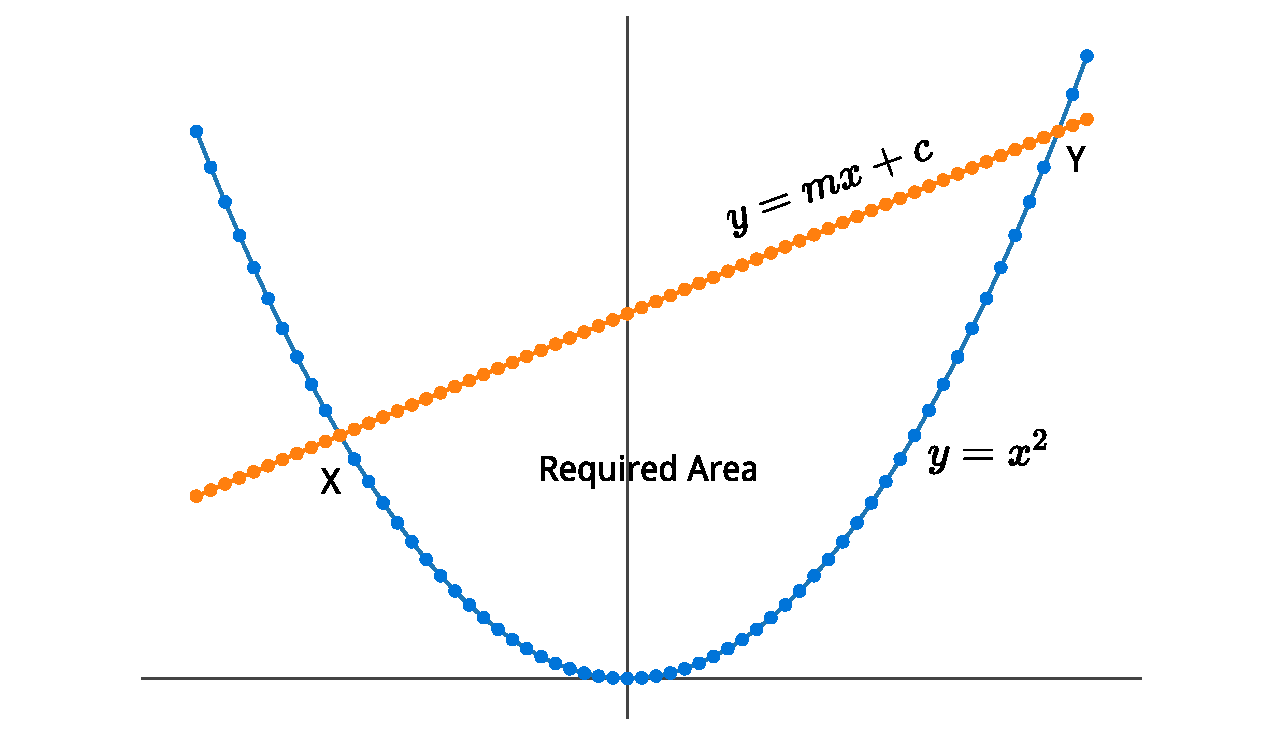
\includegraphics[width=300pt]{plotly.eps}
\fi

\begin{solution}[\halfpage]
   The two curves intersect at points $X$ and $Y$ where
   \begin{align}
      x^2 &= \vc x +\vd\implies x^2 - \vc x - \vd = 0 \\
      \text{or } x &= \va,\vb
   \end{align}
   
   And therefore, the area $A$ (see figure) is therefore,  
   \begin{align}
     A &= \int_{\va}^\vb (\vc x+\vd-x^2)\ud x \\
       &= \left[ \WRITEFRAC\vp\vq x^2+\vd x-\dfrac{x^3}{3} \right]_{\va}^\vb \\
       &= \left( \WRITEFRAC\vg\vh + \vi - \dfrac\vy{3} \right) 
       - \left( \WRITEFRAC\vj\vk + \vl - \dfrac\vx{3} \right) = \WRITEFRAC\vm\vn
   \end{align}
\end{solution}

\ifprintanswers
  \begin{codex}
    $\WRITEFRAC\vm\vn$
  \end{codex}
\fi
